% Options for packages loaded elsewhere
\PassOptionsToPackage{unicode}{hyperref}
\PassOptionsToPackage{hyphens}{url}
\PassOptionsToPackage{dvipsnames,svgnames,x11names}{xcolor}
%
\documentclass[
  a4paper,
]{article}
\usepackage{amsmath,amssymb}
\usepackage{iftex}
\ifPDFTeX
  \usepackage[T1]{fontenc}
  \usepackage[utf8]{inputenc}
  \usepackage{textcomp} % provide euro and other symbols
\else % if luatex or xetex
  \usepackage{unicode-math} % this also loads fontspec
  \defaultfontfeatures{Scale=MatchLowercase}
  \defaultfontfeatures[\rmfamily]{Ligatures=TeX,Scale=1}
\fi
\usepackage{lmodern}
\ifPDFTeX\else
  % xetex/luatex font selection
    \setmainfont[BoldFont=texgyrepagella-bold.otf,ItalicFont=texgyrepagella-italic.otf,BoldItalicFont=texgyrepagella-bolditalic.otf]{texgyrepagella-regular.otf}
\fi
% Use upquote if available, for straight quotes in verbatim environments
\IfFileExists{upquote.sty}{\usepackage{upquote}}{}
\IfFileExists{microtype.sty}{% use microtype if available
  \usepackage[]{microtype}
  \UseMicrotypeSet[protrusion]{basicmath} % disable protrusion for tt fonts
}{}
\makeatletter
\@ifundefined{KOMAClassName}{% if non-KOMA class
  \IfFileExists{parskip.sty}{%
    \usepackage{parskip}
  }{% else
    \setlength{\parindent}{0pt}
    \setlength{\parskip}{6pt plus 2pt minus 1pt}}
}{% if KOMA class
  \KOMAoptions{parskip=half}}
\makeatother
\usepackage{xcolor}
\usepackage[margin=22mm]{geometry}
\usepackage{graphicx}
\makeatletter
\newsavebox\pandoc@box
\newcommand*\pandocbounded[1]{% scales image to fit in text height/width
  \sbox\pandoc@box{#1}%
  \Gscale@div\@tempa{\textheight}{\dimexpr\ht\pandoc@box+\dp\pandoc@box\relax}%
  \Gscale@div\@tempb{\linewidth}{\wd\pandoc@box}%
  \ifdim\@tempb\p@<\@tempa\p@\let\@tempa\@tempb\fi% select the smaller of both
  \ifdim\@tempa\p@<\p@\scalebox{\@tempa}{\usebox\pandoc@box}%
  \else\usebox{\pandoc@box}%
  \fi%
}
% Set default figure placement to htbp
\def\fps@figure{htbp}
\makeatother
\setlength{\emergencystretch}{3em} % prevent overfull lines
\providecommand{\tightlist}{%
  \setlength{\itemsep}{0pt}\setlength{\parskip}{0pt}}
\setcounter{secnumdepth}{-\maxdimen} % remove section numbering
\usepackage{bookmark}
\IfFileExists{xurl.sty}{\usepackage{xurl}}{} % add URL line breaks if available
\urlstyle{same}
\hypersetup{
  colorlinks=true,
  linkcolor={Maroon},
  filecolor={Maroon},
  citecolor={Blue},
  urlcolor={Blue},
  pdfcreator={Python and XeLaTeX}}

\author{}
\date{}


\begin{document}
\section{Qiaoyi(Joyce) Xu}
\subsection{BASIC INFORMATION}
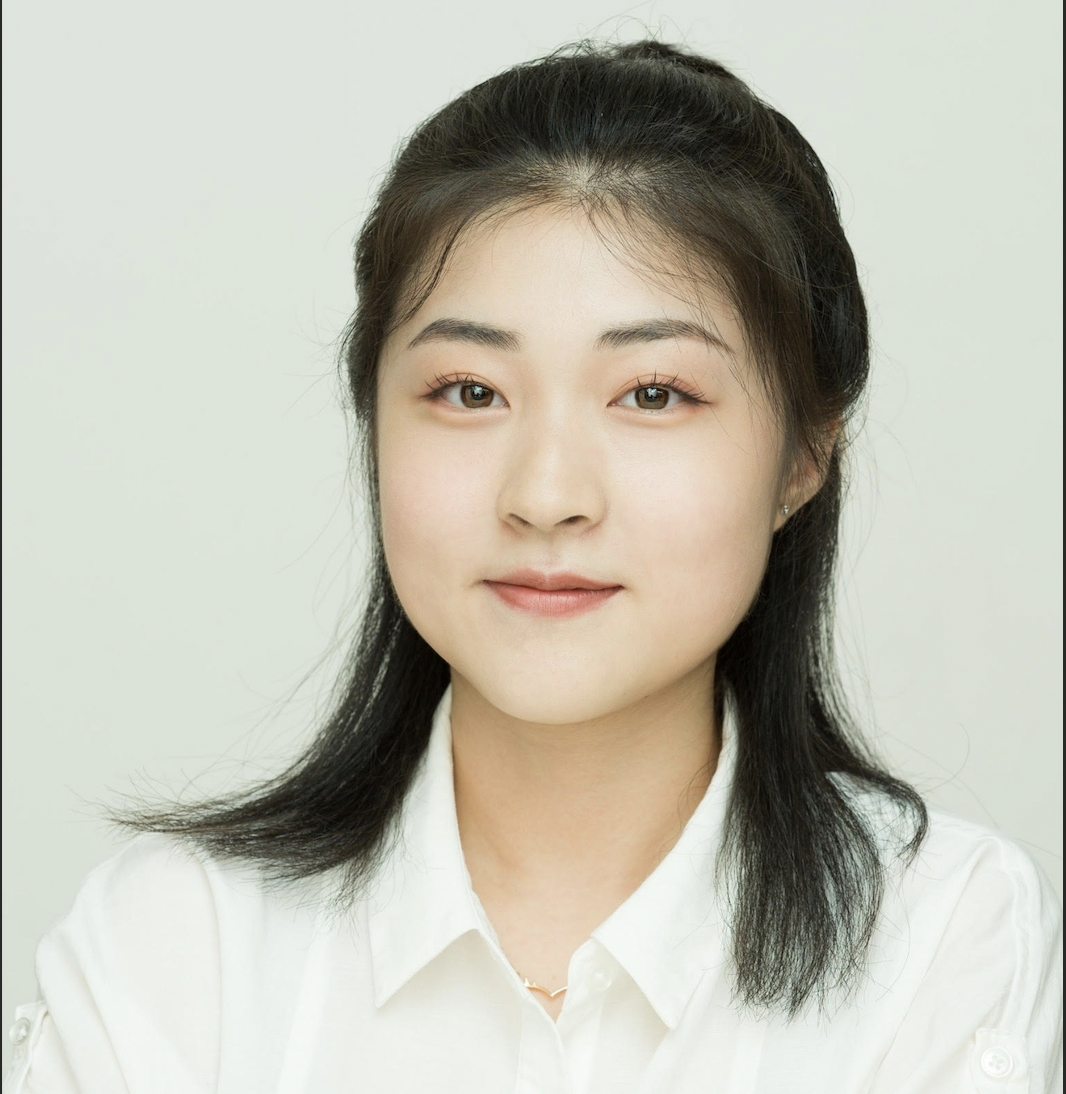
\includegraphics[width=0.4\linewidth]{portrait.jpeg}

\emph{Phone number}: +86 15711312382

\emph{Email}: \href{mailto:qiaoyixu2000@gmail.com}{qiaoyixu2000@gmail.com}

\emph{Address}: Beijing, China

\bigskip
\subsection{EDUCATION}
\textbf{Peking University, Beijing, China} \hfill Sep. 2026-Expected Jul. 2030

\emph{Doctor of Philosophy in Epidemiology and Biostatistics}

\textbf{Columbia University, New York, NY} \hfill Sep. 2021-May 2023

\emph{Master of Public Health in Epidemiolog, Certificate in Applied Biostatistics} \hfill GPA:3.93

\textbf{University of Massachusetts Amherst, Amherst, MA} \hfill Sep. 2018-May 2021

\emph{Bachelor of Science in Public Health Sciences and Mathematics, Double Major} \hfill GPA:3.8

\bigskip
\subsection{PROFESSIONAL EXPERIENCE}
\textbf{Pharmaron Clinical} \hfill July 2023-August 2026

\emph{Biostatistician}

\begin{itemize}
\tightlist
\item Participated in several clinical trial projects, including Phase I/II studies, Bioequivalence (BE) studies, Investigator-Initiated Trials (IITs), and statistical analyses for FDA IND application support. Indications include Multiple Myeloma, Transfusion-dependent β-thalassemia, Diabetic Ulcers, Psoriasis, etc.;
\item Generated critical statistical documents: statistical analysis plans (SAPs), Table, Listing, and Figure (TLF) templates, and Protocol Deviation Handling and Reporting Procedure, ensuring compliance with ICH and CDE guidelines;
\item Reviewed study protocols, programmed TLF deliverables, population definition documents, and cross-functional documents such as Case Report Forms (CRFs) and other data management-related documents.
\end{itemize}
\newpage
\textbf{Pfizer Inc, New York, NY} \hfill June-Aug. 2022

\emph{-Epidemiology Research Assistant, Medical Development and Scientific/Clinical Affairs}

\begin{itemize}
\tightlist
\item Provided critical epidemiology supports in the development of the Lyme disease vaccination
\item Conducted an individual project of Systematic Literature Review in Canada tick surveillance
\item Analyzed database used by SAS and presented results
\end{itemize}
\textbf{Frost and Sullivan, Shanghai, China} \hfill Dec. 2021-Feb. 2022

\emph{-Consulting Analyst Intern}

\begin{itemize}
\tightlist
\item Assisted in data collection for programs
\item Made slides and presentation to support market analysis of company
\item Participate in expert interviews and write interview minutes
\end{itemize}
\textbf{National Center for Medical Service Administration, Beijing, China} \hfill July-Sept. 2020

\emph{-Data Analyst Intern}

\begin{itemize}
\tightlist
\item Collected Nucleic Acid Test data from 20 hospitals/health centers everyday
\item Organized daily work dynamics and analyzed Nucleic Acid Test data
\item Write daily reports about COVID-19 according to the results of analyzing data
\end{itemize}
\textbf{Chinese Center for Disease Control and Prevention, Beijing, China} \hfill June-Aug. 2019

\emph{-Data Analyst Intern, office for major projects}

\begin{itemize}
\tightlist
\item Collected data from many different provinces about air quality and water quality
\item Analyzed prior air quality data and discussed with supervisor
\item Learned how to write report according to the results of analyzing data
\end{itemize}
\emph{-Intern, shielded room}

\begin{itemize}
\tightlist
\item Disseminate public health awareness across primary and middle school children and created poster competition for children ages 6-15, related with how to protect environment.
\item Prepared meeting that we invited many professors to have lecture about environmental health knowledge for children and parents.
\end{itemize}
\bigskip
\subsection{SKILLS}
Languages: Fluent in Mandarin Chinese and English

Technical: SAS(Advanced), R (Advanced), MySQL(advanced), Excel (Advanced)
\end{document}